\begin{figure}[H]
\centering
\begin{minipage}[t]{58mm}
\vspace{0pt}
\centering
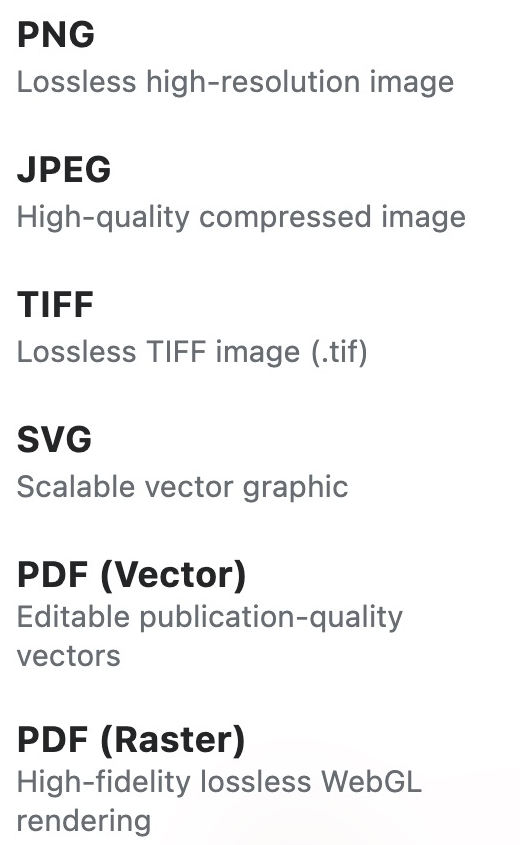
\includegraphics[width=52mm]{publication-assets/crop-496bc1fbfb3e99bfc4e7.png}
\end{minipage}\hspace{4mm}%
\begin{minipage}[t]{58mm}
\vspace{0pt}
{\centering
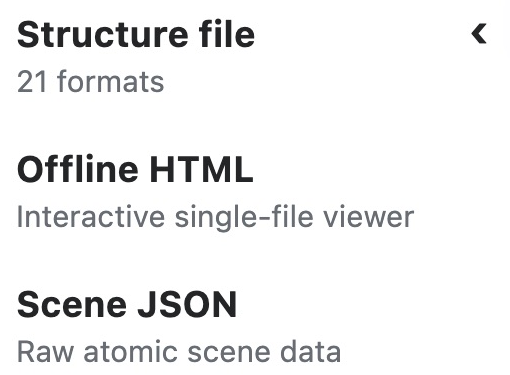
\includegraphics[width=51mm]{publication-assets/crop-68b4df9ea7d48ce9da1e.png}\par}
\par\vspace{3mm}
\raggedright\fontsize{9}{13}\selectfont
\ui{Structure file}儲存所選格式能表達的模型資訊。

\smallskip
\ui{Offline HTML}用於在本機瀏覽器中旋轉觀察。

\smallskip
\ui{Scene JSON}記錄原子場景，區別於結構JSON。
\end{minipage}
\caption{原子檢視器的兩類匯出選單。左側\ui{Export image}提供六種影象格式；右側\ui{Export file}分別通向結構檔案、離線頁面與場景JSON。}
\label{fig:atomic-export-menus}
\end{figure}
